\documentclass[a4paper,twoside,12pt,DIV=13,BCOR=5mm,numbers=noenddot,cleardoublepage=empty]{scrbook}
\usepackage[utf8]{inputenc}
%======= Einbinden der benötigten Packete (= Zusatzfunktionen)
\usepackage[T1]{fontenc}                % für Fonts in westeuropäischer Codierung
\usepackage{lmodern}										% Latin Modern Paket verändert die verwendete Schriftart. Bessere Darstellung für pdf
\usepackage{textcomp}										% Provides extra symbols, e.g. arrows like \textrightarrow, various currencies (\texteuro,..
\usepackage[latin1]{inputenc}    				% german special characters
\usepackage[english,ngerman]{babel}     % hyphenation   usepackage[english,ngerman]{babel} f. deutsch
\usepackage{pdfpages}										% Einbinden von pdf-Files
\usepackage{pifont,textcomp,mathcomp}   % dingbad psfonts and text-compilant fonts (euro, TM, ...)
\usepackage{amsmath,amsopn,amsthm}      % AMS mathematics
\usepackage{amssymb}                    % zusätzliche Symbole 
\usepackage{xspace}											% avoids eaten spaces

%======= Eine Umgebung für Bilder und Tabellen			  	
%\usepackage[textfont={Small},labelfont={bf},margin=1cm,format=plain,font=singlespacing]{caption}   % hanging caption text [hang]
\usepackage[textfont={small},labelfont={bf},margin=1cm,format=plain,font=singlespacing]{caption}   % hanging caption text [hang]
\captionsetup*[figure]{name=Abb.}			 % Abbildungsunterschrift beginnt mit Abb.
\captionsetup*[table]{name=Tab.}


%======= Farben für Überschriften
\usepackage{color}
\definecolor{TUBlau}{rgb}{0,0.4,0.6}   % TU-blau RGB 0 102 153
\addtokomafont{sectioning}{\sffamily\bfseries\selectfont\color{TUBlau}}
\setkomafont{chapter}{\normalfont\huge\sffamily\bfseries\color{TUBlau}}
\addtokomafont{section}{\Large}
\addtokomafont{subsection}{\normalfont\Large\sffamily\bfseries\color{TUBlau}}
\addtokomafont{subsubsection}{\normalfont\large\sffamily\bfseries\color{TUBlau}}
\addtokomafont{paragraph}{\normalfont\large\sffamily\bfseries\color{TUBlau}}


%======= Kopf-/Fußzeilen
\pagestyle{plain} % nur Fußzeile



%======= Eine kompakte Umgebung für die Bilder
\newcommand{\bild}[4]{{
\begin{figure}[#2]
\begin{center}
\includegraphics[scale=#3]{pictures/#1}
\caption{#4}\label{fig:#1}
\end{center}
\end{figure}
}}


%======= Definitionen eigener Befehle
\newcommand{\degC}{\ensuremath{^{\circ}}C}        % Grad Celsius
\newcommand{\Gu}{\glqq{}}                         % Gänsefüßchen unten
\newcommand{\Go}{\grqq{}\xspace}    												% Gänsefüßchen oben











  			
\usepackage{subscript}

\begin{document}

\setcounter{chapter}{0}

\chapter{Aufnahme einer Hystereseschleife}

    Die Magnetisierung beschreibt den Zusammenhang zwischen der magnetischen Flussdichte $\Vec{\textbf{B}}$ und der magnetischen Feldstärke $\textbf{H}$:
    \begin{equation}
        \textbf{B} = \mu_0 (\textbf{H} + \textbf{M}) = \mu\textbf{H}
    \end{equation} 
    Dabei ist $\mu_0$ die magnetische Feldkonstante und $\mu$ die Permeabilität. \\
    Durch eine Hystereseschleife kann die Beziehung zwischen $\textbf{B}$ und $\textbf{H}$ anschaulich präsentiert werden. Eine typische Hystereseschleife ist eine geschlossene Kurve, die im \textbf{B}-\textbf{H}-Koordinatensystem abgebildet wird. \\
    
    \begin{itemize}
        \item Wenn eine entmagnetisierte Probe bis zur positiven Sättigungsmagnetisierung $+M_S$ aufmagnetisiert wird, wird die \textbf{Neukurve} durchlaufen. Bei höheren Magnetfeldstärken wird der \textbf{Sättigungspunkt} erreicht, wo die Flussdichte nicht weiter steigen kann.
        \item Wenn das Magnetfeld in die entgegengesetzte Richtung geändert wird, sinkt die magnetische Flussdichte nicht sofort auf Null. Stattdessen bleibt eine Restmagnetisierung im Material zurück. Dieser Punkt wird als \textbf{Remanenzpunkt} mit \textbf{B$_R$} bezeichnet.
        \item Um die Restmagnetisierung zu neutralisieren und das Material vollständig zu entmagnetisieren, muss das entgegengesetzte Magnetfeld eine bestimmte Stärke erreichen. Diese Stärke wird als \textbf{Koerzitivfeldstärke} \textbf{H$_C$} bezeichnet. \\
    \end{itemize}
    
    \section{Übungsdurchführung}
    
    Im Rahmen der Laborübung war das magnetische Verhalten von unlegiertem Einsatzstahl zu bestimmen. Neben dem Eisenring wurden noch ein Funktionsgenerator und ein Integrator mit USB-Anschluss zur Verfügung gestellt. Die Hystereseschleifen wurden durch den Integrator aufgezeichnet und konnten mittels einer Software am PC zur Analyse dargestellt werden.

    \newpage
    
    \subsection{Probe}

    Zur Messung des magnetischen Verhaltens von unlegiertem Einsatzstahl wurde ein \textbf{Eisen-Ringkern} aus ungeblechtem und unlegiertem Einsatzstahl bereitgestellt, der mit vier verschiedenen Wicklungen umwickelt ist.

    \begin{center}
    \begin{tabular}{|c|c|} \hline
    Wicklung W1: & 730 Windungen \\ \hline
    Wicklung W2: & 749 Windungen \\ \hline
    Wicklung W3: & 732 Windungen \\ \hline
    Wicklung W4: & 731 Windungen \\ \hline
    Kernaußendurchmesser $d_a$: & 183 mm \\ \hline
    Kerninnendurchmesser $d_i$: & 153 mm \\ \hline
    Breite $b$: & 15 mm \\ \hline
    Höhe $h$: & 15 mm \\ \hline
    Wirksamer Querschnitt $A_w$: & 225 mm² \\ \hline
    Mittlere Eisenlänge $l_m$: & 528 mm \\ \hline
    \end{tabular}
    \end{center}
    
    \subsection{Schaltung}

    Es wurden zwei Widerstände und drei Spulen in Serie zusammengeschaltet. An \textit{$R_2$} wurde die Eingangsspannung $U_x$ gemessen. An die vierte Spule wurde der Integrator zur Messung der Ausgangsspannung $U_y$ angeschlossen.
    \begin{figure}[h] 
    \centering
    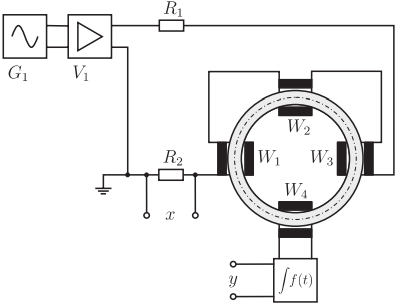
\includegraphics[width=0.5\textwidth]{pictures/HystereseSchaltung.png} % Passe die Breite des Bildes an deine Bedürfnisse an
    \caption{Schaltungsaufbau (aus dem Skript)}
    \end{figure}
    \\
    Mit $R_1$ = 4,7 $\Omega$, $R_2$ = 1 $\Omega$. \\
    Durch den Funktionsgenerator wurde ein 100 mHz, 20 Vpp Dreiecksignal eingespeist.

    \newpage

    \subsection{Messergebnisse}

        \begin{enumerate}
            \item Die Magnetisierungskurve bei 100 mHz sieht so aus:

            \begin{figure}[h] 
            \centering
            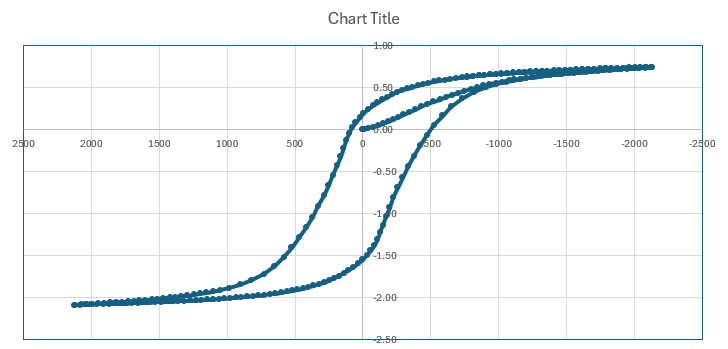
\includegraphics[width=1\textwidth]{pictures/50mHz.png} 
            \caption{Hystereseschleife, 50 mHz}
            \label{fig:meinbild}
             \end{figure}

            \\

            \item
                Die Maßstäbe der Achsen müssen aus den Spannungen $U_x$ und $U_y$ bestimmt werden:
                \begin{equation}
                    H = \frac{(N_1 + N_2 + N_3) \cdot I_1}{l_m} \\
                    = \frac{N_1 + N_2 + N_3}{R_2 \cdot l_m} \cdot U_x \\
                \end{equation}
                \begin{equation}
                    H = 4187,604 \frac{\text{A}}{\text{m}} \cdot U_x
                \end{equation}

                und die magnetische Flussdichte $B$:
                \begin{equation}
                    U_y = -\frac{1}{R \cdot C} \cdot \int U_4 \cdot dt \\
                    = \frac{1}{\tau} \cdot \int N_4 \cdot \frac{d\phi}{dt} \cdot dt \\
                    = \frac{1}{\tau} \cdot N_4 \cdot \phi \\
                    = \frac{1}{\tau} \cdot N_4 \cdot B \cdot A \\
                \end{equation}
                \begin{equation}
                    B = \frac{\tau}{N_4 \cdot A} \cdot U_y \\
                    = -547,196 \cdot 10^{-3} \frac{\text{T}}{\text{V}} \cdot U_y
                \end{equation}

            \\

            \newpage
            \item Je höher die Frequenz eingestellt ist, desto mehr wird die Hystereseschleife verzerrt. Ab einem bestimmten Punkt sind die Spitzen nicht mehr zu beobachten.

            \begin{figure}[h] 
            \centering
            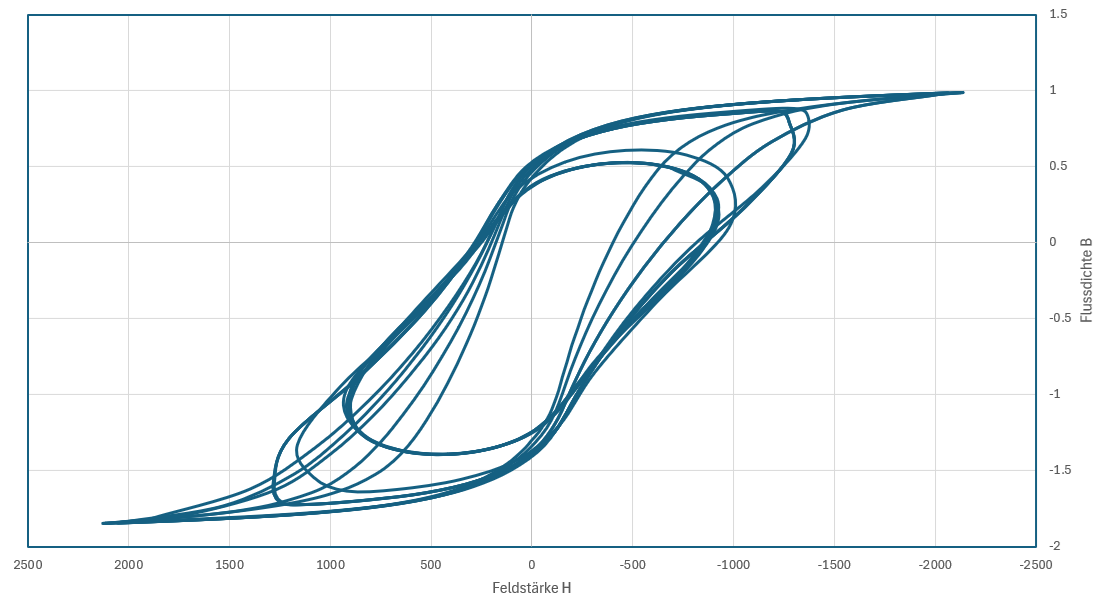
\includegraphics[width=\textwidth]{pictures/freqAnderung.png} 
            \caption{Frequenzänderung mit 100 mHz Schritten}
            \label{fig:meinbild}
            \end{figure}

            Auf der Abbildung wurde die Frequenz in 100 mHz Schritten erhöht von 100 mHz bis zu 1,3 Hz.
            
            \\

            \item Bei höheren Frequenzen haben die Magnetfeldänderungen eine größere Wirkung auf das Material. Dies kann zu verstärkten Wirbelstromverlusten führen, insbesondere in leitfähigen Materialien wie Eisenkernen. Diese Verluste beeinflussen die Form der Hystereseschleife und können dazu führen, dass sie breiter wird und die Sättigung des Materials schneller auftritt.

            \\

            \item Die Frequenz kann als passend betrachtet werden, solange die Spitzen der Magnetisierungsschleife klar erkennbar sind. In unserem Fall sind die Spitzen bei Frequenzen größer als 200 mHz nicht mehr erkennbar, daher ist die höchste geeignete Frequenz 200 mHz.

            \\

            \item Eine Stromquelle könnte verwendet werden, um den Ausgangsstrom basierend auf einer Referenz zu regeln.             
            \\

            \item Wenn man den Nullpunkt im Symmetriemittelpunkt der Hystereseschleife annimmt, können die Messwerte einfach von der Tabelle abgelesen werden. \\
            \begin{tabular}{cc}
                $B_r$ =& 1,100 T  \\
                $H_c$ =& 256 $\frac{A}{m}$ \\
                $B_{max}$ =& 0,739 T
            \end{tabular}
            
            \\
            
            \item Die magnetische Sättigung in einem Eisenkern liegt im Bereich von 1,6 bis 2,2 Tesla. Anhand der Hystereseschleife kann man sehen, dass die Flussdichte bei maximaler Feldstärke noch steigen könnte, sodass die Sättigung beim maximalen Strom nicht erreicht wurde.

            \\
            
            \item Die maximale Flussdichte ohne den Eisenkern kann durch Division mit der spezifischen Permeabilität $\mu_0$ berechnet werden:
                \begin{equation}
                B_{\text{max, ohne Kern}} = \frac{B_{\text{max, mit Kern}}}{\mu_0}
                \end{equation}
    
            \\
            
            \item Die spezifischen Verluste sind eng mit der Fläche innerhalb der Magnetisierungskurve verbunden. Die Fläche repräsentiert nämlich die Energieverluste des Materials pro Volumeneinheit pro Zyklus. Anhand des Plots sind die spezifischen Verluste 1812,5 W/kg.
        
        \end{enumerate}
    
    \end{document}